%source mathadata
\begin{multicols}{2}
		\begin{MADenumerate}

			\item On considère les points de référence $R(1;4)$ et $S(7;2)$. Dans la suite, on cherchera des points à égale distance de $R$ et de $S$ pour retrouver la séparation entre les zones d'estimation.
			\begin{enumerate}
				\item Placer les points $R$ et $S$ dans le repère.
				\item Calculer les coordonnées du milieu $M$ de $[RS]$ à l'aide de la formule.
			\end{enumerate}

			\item Choisir deux points $P$ et $Q$ dans le repère qui semblent être à égale distance de $R$ et de $S$. Ils ne doivent pas être le milieu $M$.

			\item Calculer les distances $PR$, $PS$, $QR$ et $QS$ pour vérifier les choix. Rectifier les coordonnées de $P$ et $Q$ si nécessaire pour qu'ils soient à égale distance de $R$ et de $S$.

			\item Que remarque-t-on sur les points $M$, $P$ et $Q$ ?

			\item Tracer la droite passant par les points précédents. Qu'est-ce que cette droite représente pour l'algorithme et comment l'appelle-t-on mathématiquement ?

		\end{MADenumerate}

		%\columnbreak

		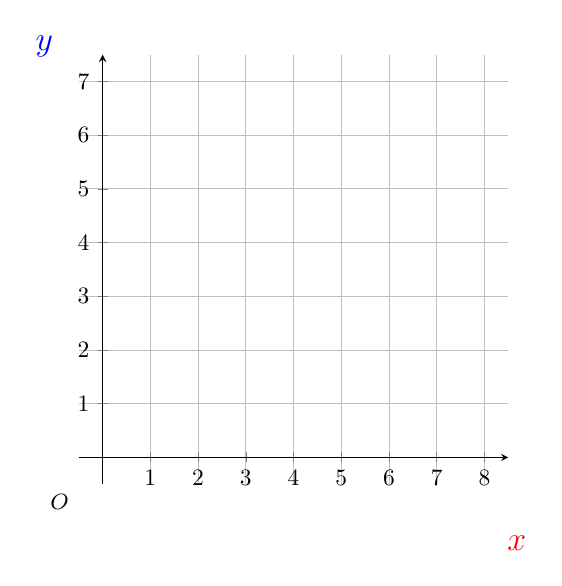
\begin{tikzpicture}[scale=0.85]
			\begin{axis}[
					name=plotMed,
					axis lines=middle,
					ymajorgrids=true,
					xmajorgrids=true,
					xmin=-0.5,
					xmax=8.5,
					ymin=-0.5,
					ymax=7.5,
					xtick={0,1,...,8},
					ytick={0,1,...,7},
					xlabel={\Large{\color{red}$x$}},
					xlabel style={at={(axis description cs:1.02,-0.1)}, anchor=north},
					ylabel={\color{blue}{\Large$y$}},
					ylabel style={at={(axis description cs:-0.12,1.02)}, anchor=west},
					width=8cm,
					height=8cm,
				]
			\end{axis}
			\draw (0,0) node[below left]{\footnotesize $O$};
		\end{tikzpicture}

	\end{multicols}
